\textbf{Overview.}
We quantize the OPT~\citep{meta2022opt} family of models (up to 66B parameters) and Llama 2 70B~\citep{meta2023llama} using various quantization and processing methods.
QuIP is superior to OPTQ and other baselines across all model sizes and evaluation tasks.
Most interestingly, incoherence processing yields excellent performance using as little as two bits per weight when paired with any of the quantization methods we consider (including nearest rounding). Two-bit quantization with QuIP is viable at even moderate model sizes (1B parameters), a regime where other two-bit quantization methods fail. At the largest model sizes, the difference between 2-bit and 16-bit weight performance becomes small.
We compare the throughput of QuIP with OPTQ's efficient implementation on language generation and show that it is not much slower.
Additional results on the effectiveness of the proxy loss, unbiased rounding, and Algorithm~\ref{alg:qcvx} are presented in the Supplement~\ref{suppAddResults}.

\textbf{Setup.} 
The experimental infrastructure is built on top of OPTQ's~\citep{frantar2023gptq} repository which is implemented in PyTorch~\citep{paszke2019pytorch}.
We quantize the HuggingFace implementations of the OPT and Llama 2 model families.
All models are quantized on a single GPU, with up to 48GB of memory.
Our calibration set is the same as OPTQ; 128 random 2048 token segments from the C4 dataset~\citep{raffel2020c4} consisting of generic text data from crawled websites.
Therefore, no task-specific data is viewed when quantizing.
Following OPTQ, quantization is performed one Transformer block at a time:
loaded into GPU memory, the Hessian computed, and then the weights quantized.
The current block's inputs are then passed through the quantized block to produce inputs for the following block.
The Hessian is computed from the quantized Transformer up to that point rather than from the full precision model;
like OPTQ, we find this improves quantization.
Further details on the setup can be found in Supplement~\ref{suppAddResults}, including a description of the computational resources used to perform the experiments.


\textbf{Methods.}
We evaluate compositions of several quantization and pre/post processing methods.
For quantization methods, we evaluate nearest rounding, LDLQ (or OPTQ), and two variations.
LDLQ-RG re-orders the weights based on $\operatorname{diag}(H)$ to modify the quantization order and adds further greedy updates to the proxy.
``Greedy'' performs the greedy updates only.
We evaluate the baseline preprocessing from OPTQ which adds $H \gets H +\alpha * \operatorname{mean}(\operatorname{diag}(H))I$
for numerical stability. 
We also evaluate our incoherence processing in Algorithms~\ref{algQuIPpre} and~\ref{algQuIPpost}, denoted as ``IncP''.
With this notation QuIP = LDLQ + IncP, and QuIP-RG = LDLQ-RG + IncP.

\textbf{Datasets.}
We evaluate 
on the following language generation tasks: WikiText2~\citep{merity2016wiki}, Penn Treebank (PTB)~\citep{marcus1994penn}, and C4.
We also evaluate on zero-shot tasks, including LAMBADA (LAMB)~\citep{paperno2016lambada}, ARC Easy (ArcE)~\citep{boratko2018arc}, PiQA~\citep{tat2003piqa}, and StoryCloze (SC)~\citep{2016storycloze}.
See Supplement~\ref{suppAddResults} for the full set of results.

\begin{figure}
\centering
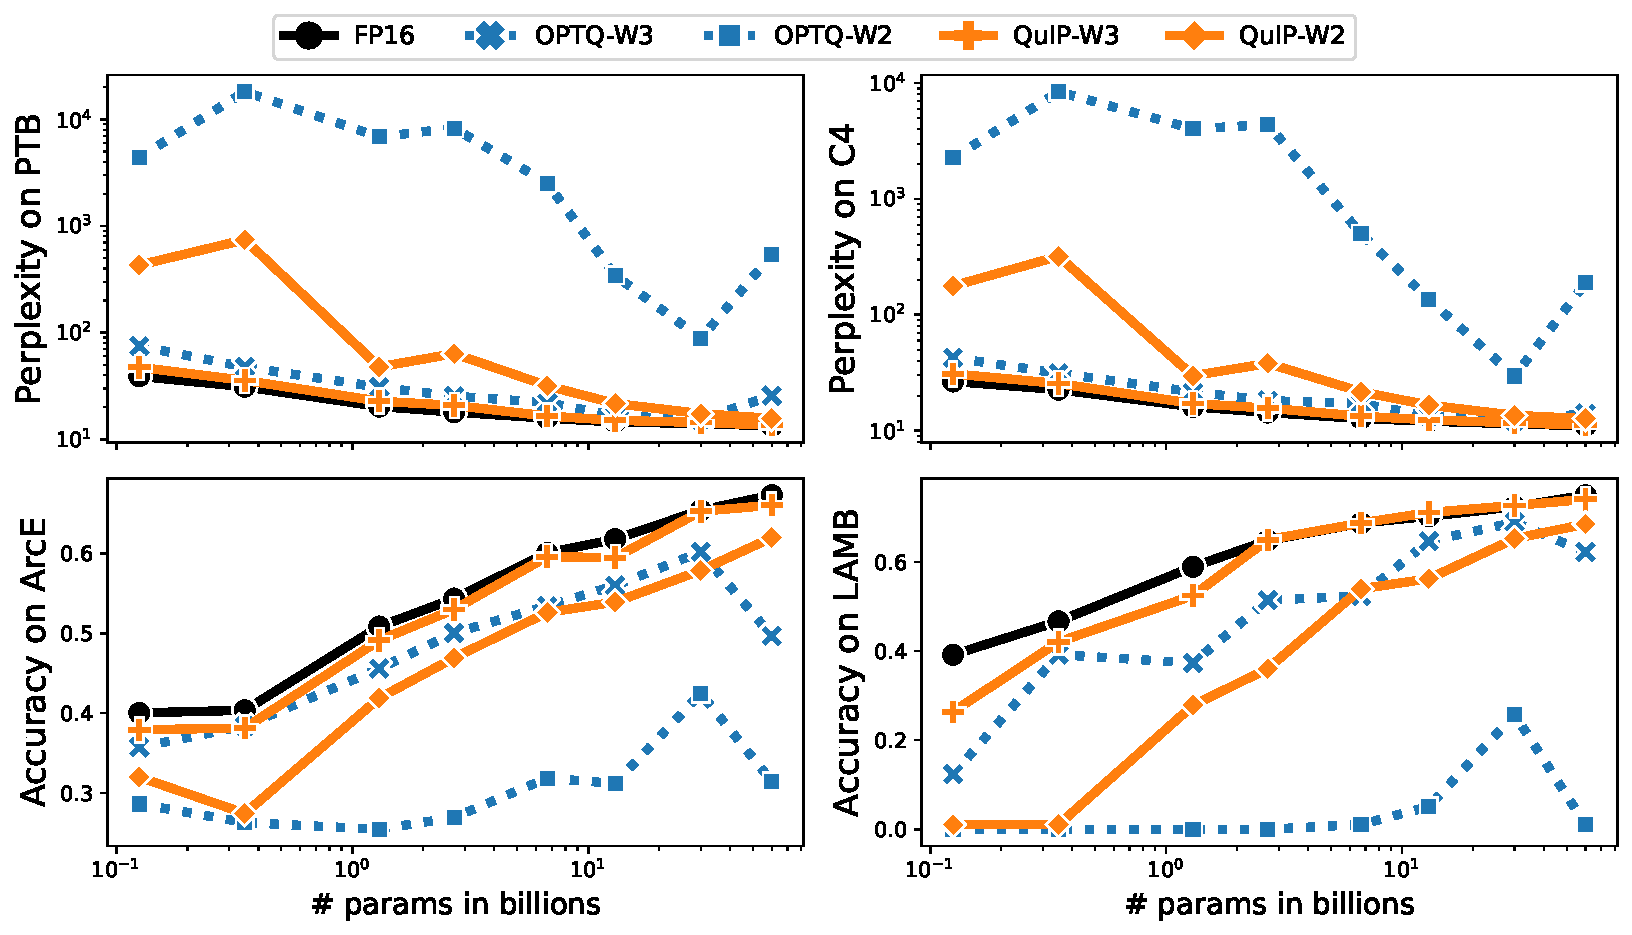
\includegraphics[width=0.92\linewidth]{figures/main_plot_newcolor.pdf}
\caption{
Quantizing OPT models up to 66B parameters.
Our method QuIP is the first PTQ procedure to achieve good quantization at 2 bits per weight, across a variety of model sizes and evaluation tasks.
}
\label{figMain}
\end{figure}

\begin{table}[]
\centering
\small
\begin{tabular}{c|ccccc|ccccc}
& \multicolumn{5}{c|}{OPTQ} & \multicolumn{5}{c}{QuIP (Ours)} \\
\hline
WBits\Tstrut\Bstrut & 
Wiki$\downarrow$ & C4$\downarrow$ & ArcE$\uparrow$ & PiQA$\uparrow$ & SC$\uparrow$ &
Wiki$\downarrow$ & C4$\downarrow$ & ArcE$\uparrow$ & PiQA$\uparrow$ & SC$\uparrow$\\
\hline
16\Tstrut & 
3.319 & 5.709 & 59.72 & 80.90 & 79.95 &
3.319 & 5.709 & 59.72 & 80.90 & 79.95 \\
\hline
4\Tstrut & 
3.596 & 5.905 & 58.96 & 80.52 & 79.12 &
3.531 & 5.869 & 59.81 & 80.47 & 79.63 \\
3 & 
4.907 & 7.099 & 54.38 & 78.56 & 77.72 &
3.853 & 6.135 & 59.81 & 80.25 & 79.31 \\
2 & 
123.908 & 70.541 & 25.34 & 50.54 & 51.75 &
\textbf{6.326} & \textbf{8.937} & \textbf{54.38} & \textbf{75.08} & \textbf{75.37} \\
\hline 
\end{tabular}
\vspace{0.2em}
\caption{
Quantizing Llama 2 70B with QuIP and OPTQ, and evaluating on language generation and zeroshot tasks.
Our incoherence processing enables a step function change in quantization at 2 bits.
}
\label{tabLlama270BRes}
\end{table}


% (125m to 30b, perplexit and zeroshot)
\begin{table}[]
\centering
\small
\begin{tabular}{c|ccccc|ccccc}
& \multicolumn{5}{c|}{Baseline Processing} & \multicolumn{5}{c}{Incoherence Processing (Ours)} \\
% \midrule
\hline
WBits\Tstrut\Bstrut & 
Wiki$\downarrow$ & PTB$\downarrow$ & C4$\downarrow$ & ArcE$\uparrow$ & LAMB$\uparrow$ & 
Wiki$\downarrow$ & PTB$\downarrow$ & C4$\downarrow$ & ArcE$\uparrow$  & LAMB$\uparrow$\\
% \midrule
\hline
16\Tstrut & 9.56 & 14.04 & 11.45 & 65.40 & 72.40 & 9.56 & 14.04 & 11.45 & 65.40 & 72.40 \\
% \midrule
\hline
& \multicolumn{5}{c|}{\underline{OPTQ}}\Tstrut & \multicolumn{5}{c}{\underline{\textbf{QuIP}}} \\
% \midrule
4 & 
9.59 & 14.22 & 11.56 & 64.77 & 72.39 & 
9.60 & 14.18 & 11.50 & 65.32 & 73.20\\
3 & 
10.32 & 15.36 & 12.23 & 60.19 & 68.89 &
9.79 & 14.37 & 11.66 & 65.28 & 72.68
\\
2 & 
71.70 & 88.19 & 29.59 & 42.47 & 25.77 &
\textbf{11.48} & 17.40 & 13.55 & 57.87 & \textbf{65.24}
\\
% \midrule
\hline
& \multicolumn{5}{c|}{\underline{LDLQ-RG}}\Tstrut & \multicolumn{5}{c}{\underline{\textbf{QuIP-RG}}} \\
4 &
9.64 & 14.20 & 11.56 & 63.76 & 71.94 &
9.66 & 14.11 & 11.51 & 64.86 & 71.86 
\\
3 &
10.31 & 15.15 & 12.15 & 63.43 & 69.78 &
9.75 & 14.44 & 11.68 & 63.51 & 71.53 
\\
2 &
49.40 & 73.45 & 29.12 & 41.20 & 26.35 &
11.68 & \textbf{16.94} & 13.44 & \textbf{59.51} & 62.31 
\\
% \midrule
\hline
& \multicolumn{5}{c|}{\underline{Greedy}}\Tstrut & \multicolumn{5}{c}{\underline{Greedy + IncP}} \\
4 &
9.69 & 14.33 & 11.59 & 63.09 & 72.37 &
9.72 & 14.23 & 11.52 & 65.99 & 71.71 
\\
3 &
13.63 & 23.05 & 16.30 & 50.51 & 56.76 &
9.92 & 14.45 & 11.71 & 63.80 & 71.38 
\\
2 &
4816.6 & 3473.81 & 3183.2 & 26.30 & 0.00 &
11.59 & 17.39 & \textbf{13.30} & 58.80 & 64.47 
\\
% \midrule
\hline
& \multicolumn{5}{c|}{\underline{Near}}\Tstrut & \multicolumn{5}{c}{\underline{Near + IncP}} \\
4 &
10.77 & 15.41 & 13.52 & 61.28 & 70.42 &
9.77 & 14.16 & 11.53 & 64.06 & 71.41
\\
3 &
1564.9 & 1526.2 & 1808.2 & 34.47 & 1.73 &
9.89 & 14.49 & 11.74 & 64.06 & 71.41
\\
2 &
41547.8 & 34348.6 & 24815.7 & 25.80 & 0.00 &
12.04 & 18.12 & 14.11 & 56.36 & 60.64
\\
% \bottomrule
\hline
\end{tabular}
\caption{
Quantizing OPT-30b with various quantization and processing methods, and evaluating on language generation and zeroshot tasks.
Our incoherence processing enables a step function change in quantization at 2 bits, across all rounding methods.
}
\label{tabMainRes}
\end{table}

\textbf{Main Results.}
QuIP is the first PTQ procedure to achieve good quantization at two bits per weight, across a variety of LLM sizes and evaluation tasks.
In Figure~\ref{figMain} we compare QuIP and OPTQ when quantizing to 2 and 3 bits per weight (4-bit quantization works equally well for both methods); we evaluate OPT models (up to 66B) on PTB, C4, ARC Easy, and LAMBADA.
QuIP is superior to OPTQ across the model sizes and evaluation tasks.
At three bits, QuIP matches the full precision model reasonably well.
At two bits and for larger LLMs (>2B parameters), QuIP begins to approach the performance of the full precision model.
As model size increases, so does the quality of QuIP's 2-bit quantization.
We provide plots on the remaining datasets in Supplement~\ref{suppAddResults}.
Note that the dip in OPTQ on OPT-66B is documented in their paper.

Table~\ref{tabLlama270BRes} shows the results of quantizing Llama 2 70B using QuIP and OPTQ. 
Again, QuIP achieves good quantization at two bits while OPTQ does not. 


\begin{table}[]
\centering
\begin{tabular}{c|cccc}
Wbits & Rescale & Incoherence & Rescale+Incoherence & Rescale+Incoherence+Quant Range \\
% \midrule
\hline
4\Tstrut & 
24.30 &
24.32 &
24.05 &
23.89 \\
3 &
32.62 &
42.28 &
31.32 &
26.36
\end{tabular}
\caption{
Ablating sub-steps of QuIP's incoherence processing, see Algorithm~\ref{algQuIPpre}.
Perplexities are averaged over WikiText2, PTB, and C4 for OPT-350m.
}
\label{tabAblateIP}
\end{table}



\begin{wraptable}{r}{0.35\textwidth}
\centering
\begin{tabular}{cc}
Method & Throughput  \\
% \midrule
\hline
QuIP\Tstrut & 81ms \\
OPTQ & 53ms \\
\end{tabular}
\caption{
Average per-token throughput (batch size 1) when generating sequences of length 128 with OPT-66B on an A6000 GPU.
}
\label{tabThroughput}
\end{wraptable}


\textbf{Incoherence Processing Ablation.}
Table~\ref{tabMainRes} shows all combinations of quantization and processing methods evaluated on OPT-30B.
At lower weight bits, QuIP's incoherence processing dramatically improves the performance of all quantization methods, across all evaluation tasks.
Remarkably, all quantization methods---even nearest---are viable at two bits with our incoherence processing.
Our modifications in QuIP-RG sometimes give an improvement over QuIP, but further study is required to evaluate these modifications.
Figures for OPT-125M to 13B are in Supplement~\ref{suppAddResults}.

\textbf{Throughput Comparison.}
We evaluate the additional overhead of our incoherence processing during model inference by modifying OPTQ's efficient forward pass.
OPTQ's implementation contains a quantized-matrix full-precision-vector product kernel and was shown to offer speedups over a FP16 baseline.
Our incoherence processing additions are performed in PyTorch.
Table~\ref{tabThroughput} shows that our QuIP implementation is about 1.5$\times$ slower than OPTQ.





\textbf{Further Ablation.}
QuIP's incoherence processing contains several sub-steps.
Table~\ref{tabAblateIP} shows their relative contributions; all are necessary for the full improvement.
Table~\ref{tabAblateRandPermute} shows that the random permutation step within the fast orthogonal multiplication also significantly reduces perplexity.

\begin{wraptable}{r}{0.35\textwidth}
\centering
\begin{tabular}{cc}
\multirow{2}{*}{Wbits} & $\Delta$Perplexity from  \\
& random permute$\downarrow$ \\
% \midrule
\hline
4\Tstrut & -0.22 \\
3 & -9.96 \\
2 & -74.2
\end{tabular}
\caption{
Ablating random permutation within fast orthogonal multiplication.
Differences in perplexity are averaged over WikiText2, PTB, and C4 for OPT-125m.
}
\label{tabAblateRandPermute}
\end{wraptable}
